\documentclass[times, utf8, zavrsni]{fer}
\usepackage{booktabs}
\usepackage{graphicx}
\graphicspath{{./images/}}

\begin{document}

% TODO: Navedite broj rada.
\thesisnumber{5672}

% TODO: Navedite naslov rada.
\title{Sustav za upravljanje i pretraživanje baze PDF dokumenata}

% TODO: Navedite vaše ime i prezime.
\author{Luka Čupić}

\maketitle

% Ispis stranice s napomenom o umetanju izvornika rada. Uklonite naredbu \izvornik ako želite izbaciti tu stranicu.
\izvornik

% Dodavanje zahvale ili prazne stranice. Ako ne želite dodati zahvalu, naredbu ostavite radi prazne stranice.
\zahvala{}

\tableofcontents

\chapter{Uvod}
Područje analize i pretraživanja teksta neizbježno je u današnjem svijetu tehnologije. Od internetskih tražilica koje pretražuju enormne količine podataka baziranih na zadanom upitu, osobnih pomoćnika na pametnim mobitelima koji procesiraju izgovorene riječi pa sve do analize i prepoznavanja \textit{spam} elektroničkih poruka.
Kratki osvrt na ove te mnoge druge primjene ukazuju na nepobitnu činjenicu da je pretraživanje teksta...

\chapter{Pregled područja}
Korištenje računala za povrat informacija (engl. \textit{information retrieval}) datira sve do četrdesetih godina dvadesetog stoljeća, daleko prije komercijalizacije računala, odnosno njihovog korištenja u osobne svrhe. Pogledamo li samo neke od relevantnih problema poput digitalizacije knjižnica i automatizacije knjižničnih poslova, statističku analizu tekstualnih podataka u svrhe X, procesiranje korisničkih upita kako bi se pronašli relevantni dokumenti, ... Očito je da je područje analize i pretraživanja teksta vrlo zastupljeno u današnjem digitalnom svijetu u kojem se količina informacija povećava za X posto svake godine (referenca na paper), očito je da je domena primjene vrlo široka te da su analiza i pretraživanje teksta praktički zastupljeni u svakom većem području koje iziskuje nekakvu vrstu analize i pretraživanja teksta odnosno povrata informacija.

\chapter{Model dokumenata}
\label{docmodel}

\section{Prikaz dokumenata}
Prije svega, valja definirati što u kontekstu analize i pretraživanja teksta predstavlja dokument. Neformalno dokument možemo definirati kao kolekciju riječi. Ovakva kolekcija ne mora nužno biti skup, pošto dokument može imati više ponavljanja istih riječi (ova će činjenica doći do izražaja u \textbf{poglavlju X}). No ipak, za predstavljanje dokumenata biti će korišten tzv. model vreće riječi (engl. \textit{bag of words model}) kod kojeg nam nije bitna semantika samih dokumenata, pa čak niti poredak riječi, već je bitno samo pojavljuju li se riječi u određenom dokumentu, odnosno koja je učestalost njihovog pojavljivanja.
Model vreće riječi zamišljen je tako da se na početku iz svih dokumenata iz kolekcije dokumenata (u daljnjem tekstu: zbirka) izvade sve riječi te potom uklone nebitne riječi (o kojima će više riječi biti u poglavlju \ref{chap:impl}) a od preostalih se riječi izgradi vektor koji će \textit{de-facto} predstavljati dokument. Ovakav prethodno opisani model često je korišten u području procesiranja prirodnog jezika te povrata informacija kako iz dokumenata tako iz drugih tekstualnih izvora.

Da bi se dokumenti mogli predstaviti u obliku vreća riječi, potrebno je odrediti vokabular—skup svih riječi koje se nalaze u svim dokumentima promatrane zbirke. Iz ovako zadanog vokabulara potrebno je ponajprije ukloniti sve zaustavne riječi (engl. \textit{stop words})—riječi koje su učestale u nekom jeziku te su stoga nebitne za sam postupak analize teksta. Primjeri nekih zaustavnih riječi u hrvatskom jeziku su: \textit{aha}, \textit{nešto}, \textit{okolo} te \textit{zaboga}. Osim zaustavnih riječi, dodatna obrada teksta može se obaviti tzv. \textit{stemanjem} (engl. \textit{stemming}). Ova metoda ima zadaću svesti riječi na njihov kanonski oblik; nebitno je je li riječ napisana u jednini ili množini ili pak u kojem je padežu već je bitan samo kanonski oblik riječi. Na primjer, riječi poput \textit{spavao} i \textit{spavati} biti će svedene na kanonski oblik \textit{spavanje}.
Nakon stvaranja vokabulara te predobrade dokumenata (izbacivanje zaustavnih riječi, stemanje) sljedeći korak je predstavljanje dokumenata. Radi praktičnosti, najčešća metoda predstavljanja dokumenata je uz pomoć vektora.
Najjednostavnija metoda vektorskog predstavljanja dokumenata jest binarna: za svaku riječ iz vokabulara naprosto se provjeri nalazi li se u danom dokumentu te ukoliko se nalazi, odgovarajuća komponenta vektora (indeks riječi u vokabularu) biti će 1, a u suprotnom 0. Primjerice, za dokumente $d_{1}$ = "Marko jako voli domaćice. Domaćice su dobre." te $d_{2}$ = "Marko voli domaćice i programiranje.", vokabular će nakon uklanjanja svih nebitnih znakova i stop riječi biti: V = \{"Marko", "jako", "voli", "domaćice", "dobre", "programiranje"\}. Koristeći binarnu metodu reprezentacije dokumenata, odgovarajući vektori će iznositi
\begin{equation}
{{d_{1}}=[1, 1, 1, 1, 1, 0]},
\end{equation}
\begin{equation}
{{d_{2}}=[1, 0, 1, 1, 0, 1]}
\end{equation}
zbog toga što prvi dokument ne sadrži riječ "programiranje" (zadnja komponenta) dok drugi dokument ne sadrži riječi "jako" (druga komponenta) te "dobre" (predzadnja komponenta).
Nadograđujući se na prethodnu metodu, dolazi se do frekvencijskog prikaza vektora. Umjesto obične binarne reprezentacije u kojoj se pamti samo nalazi li se riječ u dokumentu ili ne, u frekvencijskom prikazu pamti se i koliko se puta dotična riječ pojavljuje u dokumentu; komponente vektora zapravo su frekvencija (tj. broj) pojavljivanja određene riječi u dokumentu. Gledajući isti vokabular i dokumente kao u prethodnom primjeru, novi vektori će u ovom slučaju iznositi:
\begin{equation}
{{d_{1}}=[1, 1, 1, 2, 1, 0]}
\end{equation}
\begin{equation}
{{d_{2}}=[1, 0, 1, 1, 0, 1]}
\end{equation}
Valja uočiti da je jedina razlika u odnosu na prethodni primjer četvrta komponenta prvog vektora koja zapravo ukazuje na to da se riječ "domaćica" u prvom dokumentu pojavljuje dvaput.
Naposlijetku dolazimo i do najčešće metode vektorskog prikaza dokumenata — TF-IDF (engl. \textit{term frequency–inverse document frequency}). Ova metoda zasniva se na dvije intuitivne pretpostavke:
\begin{itemize}
\item[$\bullet$] riječ je važnija za semantiku dokumenta što se češće u njemu pojavljuje (TF komponenta)
\item[$\bullet$] riječ je manje važna za semantiku dokumenta što se češće pojavljuje u drugim dokumentima (IDF komponenta)
\end{itemize}
TF i IDF dakle predstavljaju dvije komponente vektora kojima ćemo predstavljati dokumente. Prva komponenta je već spomenuta, frekvencija pojavljivanja riječi \textit{w} u dokumentu \textit{d}, odnosno $f_\textit{w, d}$, dok je druga komponenta obrnuta frekvencija pojavljivanja riječi u cijeloj zbirci.
Za riječ \textit{w} i dokument \textit{d}, TF i IDF komponene računaju se na sljedeći način:
\begin{equation}
{\displaystyle \mathrm {tf} (t,d)=f_{t,d}}
\end{equation}
\begin{equation}
{\displaystyle \mathrm {idf} (t,D)=\log {\frac {N}{|\{d\in D:t\in d\}|}}}
\end{equation}

Formula za TF komponentu je intuitivna i trivijalna. Formula za IDF komponentu zahtjeva kratki osvrt: riječ će biti bitnija za neki dokument što se rijeđe pojavljuje u drugim dokumentima. Odnosno drugim riječima: riječ će biti manje bitna za neki dokument što se češće pojavljuje u drugim dokumentima. Ovo ima smisla zato što neke riječi mogu biti česte u dokumentima čisto zbog same prirode jezika pa stoga ima smisla takve riječi manje uzimati u obzir prilikom računanja relevantnosti dokumenata. Dakle: što je riječ češća u ostalim dokumentima, IDF vrijednost se smanjuje te riječ postaje manje bitna za neki dokument. Naposlijetku, cijeli se omjer logaritamski skalira kako bi se u smanjio utjecaj velikog i/ili malog broja dokumenata koji sadrže određenu riječ. U nastavku je prikazan primjer izračuna TF-IDF vektora za prethodno prikazane dokumente ${d_1}$ i ${d_2}$: JE LI OVO BITNO ???

\section{Semantička sličnost dokumenata}]
\label{subchap:similarity}
Nakon izgrađene vektorske reprezentacije svih dokumenata zbirke, sljedeći korak jest samo uspoređivanje dokumenata. U sklopu ovog završnog rada, uspoređivanja dokumenata ostvaruje se na dva semantički različita načina: uspoređivanje korisničkog unosa (engl. \textit{user input}, \textit{query}) sa zbirkom dokumenata odnosno uspoređivanje pojedinog dokumenta sa zbirkom dokumenata.
Ova dva, naizgled različita problema, zapravo se svode na jedan: uspoređivanje kolekcije riječi sa zbirkom dokumenata. Ideja je dakle sljedeća: gleda se koliko riječi (bilo iz korisničkog unosa, bilo iz dokumenta, u daljnjem tekstu: ulazni vektor) iz ulaznog vektora odgovara riječima iz vokabulara, tj. koliko riječi iz ulaznog vektora odgovaraju riječima iz pojedinih dokumenata u zbirci. Što je veća korespondencija određenog ulaznog vektora s vektorom pojedinog dokumenta (tj. što više riječi dijele zajedno), to kažemo da su ta dva dokumenta sličnija. Primjerice, ukoliko se u zbirci nalazi dokument o Zvjezdanim Ratovima, a kao ulazni vektor dovedemo frazu poput "May the Force be with you", taj ulazni vektor i taj dokument imati će određenu (potencijalno visoku) mjeru sličnosti — što nas dovodi do same definicije:
\newline
Mjeru sličnosti dokumenata (engl. \textit{document similarity}) definiramo kao vrijednost na skupu pozitivnih realnih brojeva, koja ukazuje na to koliko su dva dokumenta slična — što je brojka veća, dokumenti su sličniji.
U nastavku će se razmotriti nekoliko metoda za izračun mjere sličnosti dokumenata.

\subsection{Metoda kosinusne sličnosti}
Kako su dokumenti zapravo predstavljeni vektorima u više-dimenzijskom prostoru, nad takvim dokumentima (odnosno njihovim vektorima), možemo primijenjivati operacije linearne algebre, odnosno vektorske operacije. Počevši od definicije skalarnog umnoška dvaju vektora
\begin{equation}
\mathbf {a} \cdot \mathbf {b} =\left\|\mathbf {a} \right\|\left\|\mathbf {b} \right\|\cos \theta,
\end{equation}
dolazimo do mjere kosinusne sličnosti dvaju vektora (dokumenata):
\begin{equation}
{\text{similarity}}=\cos(\theta )={\mathbf {A} \cdot \mathbf {B}  \over \|\mathbf {A} \|\|\mathbf {B}\|}
\end{equation}
Naime, sličnost dvaju dokumenata u ovom kontekstu prikazujemo kao vrijednost kosinusa kuta između njihovih vektora. Što su dokumenti sličniji, kosinus kuta biti će bliži jedinici, odnosno što su dokumenti različitiji, kosinus kuta biti će bliži nuli. Intuicija ovoga je sljedeća: ukoliko radi jednostavnosti zamislimo da vektori imaju samo dvije dimenzije, tada će sličnost dokumenata koje predstavljaju biti to veća što su oni "bliži" u 2D koordinatnom sustavu, tj. što je kosinus kuta među njima manji. Vrijedi i da će dokumenti biti manje slični što je kosinus kuta njihovih vektora veći. Grafička interpretacija prikazana je na slici
\ref{fig:vectors}.

\begin{figure}
\makebox[\textwidth]{\includegraphics[width=\textwidth]{vectors.png}}
\caption{Prikaz sličnosti dvaju vektora u 2D koordinatnom sustavu}
\label{fig:vectors}
\end{figure}

Ovo saznanje o kosinusnoj mjeri sličnosti dokumenata možemo iskoristiti u izgradnji sljedećeg modela: Neka je $v_{d_i}$ vektorska reprezentacija (binarna, frekvencijska ili TF-IDF) dokumenta $d_{i}$. Tada se sličnost dvaju dokumenata mjeri kao:
\begin{equation}
{\displaystyle {\text{similarity}}(d_{i}, d_{j})}={\frac{v_{d_i} \cdot v_{d_j}}{||v_{d_i}|| \cdot ||v_{d_j}||}}
\end{equation}
Pošto se skalarni produkt dva vektora svodi na sumu umnožaka pripadajućih komponenti (prva s prvom, druga s drugom itd.), ovo intuitivno možemo zamisliti tako da naprosto zbrajamo korespondencije odgovarajućih riječi te na kraju dijelimo sve s umnoškom njihovih normi kako bi normalizirali rezultat na interval [0, 1]. Ako se riječ nalazi u oba dokumenta, tada će taj umnožak biti pozitivan te će se pridodati mjeri sličnosti, odnosno povećati ju. Ako neka riječ ne postoji u dokumentu, tada će taj umnožak biti nula pa će automatski sličnost biti manja. Iz činjenice da je mjera sličnosti dokumenata za metodu kosinusne sličnosti definirana na intervalu [0, 1] slijedi da će dva dokumenta biti posve različita (tj. neće imati nikakvih sličnosti) ako je njihova mjera sličnosti jednaka nuli, odnosno da će dva dokumenta biti jednaka ako im je mjera sličnosti jednaka 1.

\subsection{Metoda Okapi BM25}
Za razliku od metode kosinusne sličnosti, BM25 je funkcija rangiranja koja ima za zadaću direktno rangirati dokumente po relevantnosti određenom korisničkom upitu. Iako na prvi pogled ove dvije metode izgledaju različito, zapravo se svode na istu stvar pošto je dokument zapravo samo poopćeni oblik korisnikovog upita (više o tome u poglavlju \ref{chap:impl}).
Za dokument $Q$, koji sadrži riječi $q_{1}$,...,$q_{n}$, BM25 mjera sličnosti nekog dokumenta $D$ iz zbirke računa se kao:
\begin{equation}
{\displaystyle {\text{score}}(D,Q)=\sum _{i=1}^{n}{\text{IDF}}(q_{i})\cdot {\frac {f(q_{i},D)\cdot (k_{1}+1)}{f(q_{i},D)+k_{1}\cdot \left(((1-b+b\cdot {\frac {|D|}{\text{avgdl}}}\right)}},}
\end{equation}
gdje je ${\displaystyle f(q_{i},D)}$	 frekvencija od ${\displaystyle q_{i}}$ u dokumentu D, ${\displaystyle |D|}$ je broj riječi u dokumentu D, a avgdl je prosječan broj riječi u dokumentima iz zbirke. ${\displaystyle k_{1}}$ i $b$ slobodni su parametri koji se uglavnom uzimaju kao ${\displaystyle k_{1}\in [1.2,2.0]}$ te ${\displaystyle b=0.75}.{\displaystyle {\text{ IDF}}(q_{i})}$ je IDF vrijednost komponente ${\displaystyle q_{i}}$.
Analizirajući prethodnu formulu, može se zaključiti kako metoda BM25 nema zatvoreni interval sličnosti, u odnosu na metodu kosinusne sličnosti za koju se sličnost definira na intervalu [0, 1]. Naime, koristeći metodu BM25 jedino što se može zaključiti o odnosu ulaznog vektora i pojedinog dokumenta zbirke jest kakva je mjera njihove sličnosti u odnosu da mjeru sličnosti istog ulaznog vektora i nekog drugog dokumenta iz zbirke. Dakle, pošto metoda BM25 nema ograničeni interval za mjeru sličnosti, jedina njezina svrha u ovom kontekstu jest rangiranje dokumenata po sličnosti. Ovaj će nedostatak metode BM25 doći do izražaja u poglavlju \ref{chap:impl}.

\chapter{Prikaz dokumenata u 2D koordinatnom sustavu}
Kako prethodno navedene metode ispituju sličnost različitih dokumenata, sljedeći prirodan korak bio bi vizualizacija  sličnosti dobivene među dokumentima. Ovdje međutim, nastaje jedan problem. Naime, dokumenti čija se međusobna sličnost želi prikazati grafički, predstavljeni su vektorima sačinjenim od onoliko komponenata kolika je veličina vokabulara. Uzmemo li kao primjer prosječnu duljinu znanstvenog rada koja je po PAPER tipično između 3.000 te 10.000 riječi, to bi značilo kako se i veličina vokabulara takve zbirke dokumenata također mjeri u tisućama riječi. Pošto je magnituda svakog od vektora (tj. broj komponenata) upravo veličina vokabulara, to bi značilo da svaki vektor ima tisuće komponenata koje je nemoguće prikazati u 2D ili 3D koordinatnom sustavu u svrhu vizualizacije sličnosti dokumenata. Tom se problemu u sklopu ovog rada doskače silom usmjerenim crtanjem grafova (engl. \textit{force-directed graph drawing}).

\section{Silom usmjereno crtanje grafova}
\label{subchap:forcedir}
Silom usmjereno crtanje grafova jedna je od metoda crtanja grafova koja se oslanja na simuliranje fizikalne pojave privlačnih i odbojnih sila među česticama. Naime, čvorovi grafa predstavljeni su metalnim prstenovima dok su bridovi predstavljeni oprugama. Opruge koja spajaju prstenove imaju ulogu privlačne sile (Hookeov zakon), dok je odbojna sila zapravo električna sila između prstenova. Algoritam funkcionira tako da se u svakom koraku za neki čvor odredi rezultantna sila prema svim ostalim čvorovima te se čvor pomiče u tom smjeru za određeni korak. Ovaj se postupak u svakom koraku ponavlja za sve čvorove te je cilj algoritma minimizirati ukupnu energiju sustava što će se dogoditi kada se privlačne i odbojne sile svih čvorova izjednače, odnosno kada algoritam odradi maksimalan broj koraka (koji se zadaje kao parametar algoritma).

\section{Grupiranje dokumenata}
Jedna od često korištenih metoda u kontekstu analize i pretraživanja teksta jest grupiranje dokumenata (engl. \textit{document clustering}). Cilj grupiranja jest izdvojiti dokumente neke zbirke u grupe tako da su dokumenti u jednoj grupi na neki način međusobno slični. Primjer jedne grupe dokumenata bili bi dokumenti o nogometu, košarci i odbojci pošto se sva tri dokumenta tiču sportskih aktivnosti. Kako bi se dokumenti mogli svrstati u grupe, potrebno je iskoristiti neki od algoritama za grupiranje. Jedan takav algoritam jest grupiranje k-sredina (engl. \textit{k-means clustering}).

\subsection{Grupiranje k-sredina}
Cilj ovog algoritma jest grupirati dokumente u \textit{k} grupa na način da svakom dokumentu—točki koja ga predstavlja—dodijeli grupu do čijeg je centra ta točka najbliža. Algoritam započinje tako da slučajnim mehanizmom odabere \textit{k} grupa te dodijeli dokumente u najbliže im grupe. Nakon inicijalne dodjele u grupe, računa se novih \textit{k} grupa te se postupak iterativno ponavlja do konvergencije. Nakon završenog algoritma, svaki će se dokument nalaziti u najbližoj mu grupi, zajedno s ostalim dokumentima koji su mu najsličniji. Demonstracija algoritma prikazana je na SLICI.

\begin{figure}
\makebox[\textwidth]{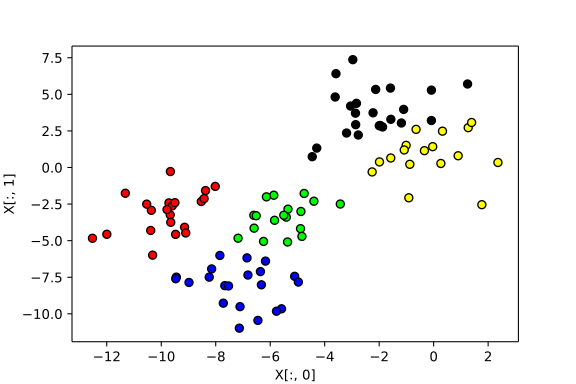
\includegraphics[width=\textwidth]{clustering.png}}
\caption{Demonstracija algoritma grupiranja}
\end{figure}

Nažalost, grupiranje dokumenta u ovome kontekstu nije izravno moguće zbog toga što algoritam apriorno (lat. \textit{a priori}) nema informaciju o broju grupa dokumenata iz zbirke. Razlog tome jest sama priroda problema koji se rješava, a to je da su na početku nepoznate grupe dokumenata (kao i njihov broj), odnosno jedini podaci dostupni programu su sami dokumenti. No ipak, broj grupa zbirke, \textit{k}, ipak se može procijeniti određenim heuristikama. Heuristika koja se koristi u ovom radu je sljedeća:
\begin{equation}
{k}={\mathbf {\sqrt{|D| \over 2}}}
\end{equation}
Ovakva heuristika ne dovodi nužno do optimalnog rješenja (tj. do egzaktnog broja grupa), no služi kao relativno dobra aproksimacija, što je u ovome kontekstu često puta sasvim dovoljno.

\section{Primjena na prikaz dokumenata}
Prethodno definirane metode (silom usmjereno crtanje grafova te grupiranje k-sredina) mogu se elegantno iskoristiti upravo za prikaz i grupiranje dokumenata, odnosno njihovih međusobnih sličnosti u 2D koordinatnom sustavu. Za svaki par dokumenata $d_{i}$ i $d_{j}$, $i \neq j$, izračuna se njihova sličnost (koristeći neku od metoda prikazanih u potpoglavlju \ref{subchap:similarity}) te se čvorovi (dokumenti) i bridovi (sličnosti) predaju algoritmu koji odsimulira postupak opisan u potpoglavlju \ref{subchap:forcedir}. te nakon određenog broja koraka, postupak prestaje i prikazuje nacrtani graf.
Nad tako nacrtanim grafom dalje se primjenjuje algoritam grupiranja k-sredina koji procijenjuje hiperparametar \textit{k} uz pomoć već opisane heuristike te provodi postupak grupiranja. Nakon što se oba algoritma izvrše, dobiveni rezultat jest upravo prikaz dokumenata u 2D koordinatnom sustavu s naznačenim grupama koje predstavljaju aproksimaciju broja kategorija dokumenata iz zbirke.

\chapter{Isprobavanje metoda...}
Jedan od ciljeva ovog rada jest istražiti već ranije spomenute metode analize i pretraživanja teksta.

Prilikom istraživanja različitih metoda rangiranja za potrebe ovog rada, metode koje su se pokazale najzanimljivijima (a koje su svejedno poprilično bazične, u smislu da ne iziskuju kompleksnije alate poput strojnog učenja) su metoda kosinusne sličnosti te metoda Okapi BM25.

\chapter{Programsko rješenje}
\label{chap:impl}
Programske potpora kao implementacija ovog završnog rada napisana je u programskom jeziku Java. Razlog ovakvog odabira leži u tome što je Java popularan i efikasan objektno orijentirani jezik zbog čega je idealan za rješavanje problema iz domene analize i obrade teksta zbog svoje objektne metodologije, nativne podrške apstraktnih kolekcija podataka, mogućnosti korištenja raznih vanjskih biblioteka itd. \newline \newline
Kao što je već ranije spomenuto, pročitani dokumenti reprezentirani su vektorima obzirom da je to najjednostavniji i najefikasniji način prikaza dokumenata. Naime, u memoriji se na taj način ne trebaju eksplicitno spremati riječi za svaki dokument već se mogu spremiti samo brojke koje govore koliko je dotična riječ relevantna za dokument. Kako se u sklopu ovog rada koristi TF-IDF reprezentacija dokumenata, to znači da se za svaki dokument treba izračunati njegova TF-IDF (vektorska) reprezentacija. Prije samog izračuna komponenata TF-IDF vektora, trebaju se pročitati PDFdokumenti smješteni na disku, pošto se u sklopu ovog rada radi s PDF dokumentima. Pošto su PDF dokumenti zapravo binarne datoteke, po svojoj strukturi nisu trivijalno parsabilni, zbog čega se za njihovo čitanje, odnosno parsiranje koristi vanjska biblioteka Apache PDFBox koja iz zadanog PDF dokumenta ekstrahira Unicode znakove koje može pročitati te ih vrati kao rezultat. Dobiveni tekst se, iz tako pročitanih dokumenata, dodatno obrađuje pri čemu se uklanjaju bilo kakvi interpunkcijski znakovi, dijakritici, brojke, odnosno svi znakovi koji nisu mala ili velika slova engleske abecede. Ovakav postupak nužan je za što točnije uspoređivanje dokumenata.
Jednom kada je tekst isfiltriran, nad njim se provodi daljnja predobrada koja: 1) uklanja iz teksta stop-riječi te 2) vrši stemanje nad dobivenim riječima dokumenata. Nakon završene predobrade teksta, stvaraju se vokabular, vektori (za reprezentaciju dokumenata) te nekoliko dodatnih pomoćnih struktura podataka. Nakon ovog koraka vrši se još i izračun sličnosti dokumenata kako bi jednom izračunati podaci bili spremljeni za ponovno korištenje. Kako bi upiti korisnika bili što optimiraniji, nakon što se prvi put izvrši čitav gore opisan postupak (preprocesiranje dokumenata, stvaranje vokabulara, računanje sličnosti dokumenata itd.), dobiveni se podaci sprema u keš (engl. \textit{cache}) memoriju, odnosno serijaliziraju (engl. \textit{serialization}) se na disku. Svrha ovog postupka jest jednom dobivene i izračunate relevantne podatke zbirke dokumenata te ih spremiti u perzistentnu memoriju računala kako bi se po svakom sljedećem pokretanju programa, umjesto ponovnog prikupljanja i izračuna svih relevantnih podataka, podaci mogli efikasnije isčitati iz zapisane datoteke te deserijalizirati u odgovarajuće strukture podataka čime se uvelike dobija na brzini izvođenja programa, kao što se može vidjeti u Tablici
\ref{table:serialization} u kojoj je vidljivo da se korištenjem serijalizacije postiže prosječno ubrzanje od čak 58 puta prilikom svakog (ne-inicijalnog) pokretanja programa.

\section{Procesiranje i obrada korisničkog unosa}
Programsko rješenje ovog završnog rada nudi korisniku interaktivan način pretraživanja postojeće zbirke dokumenata postavljanjem upita kroz grafičko korisničko sučelje. Naime, nakon postavljene putanje do zbirke dokumenata, korisnik postavlja upit te program pretražuje zbirku i korisniku prikazuje dokumente sortirane po relevantnosti korisničkom upitu. Korisnički se upit procesira kao što je već ranije spomenuto u poglavlju \ref{docmodel}: zanemaruju se svi znakovi koji nisu slova engleske abecede, uklanjaju se stop riječi, provodi se stemanje te se nakon toga korisnički unos procesira. Naime, za svaku riječ provodi se metoda kosinisne sličnosti odnosno BM25 te se od korisničkog unosa dobije vektor koji taj unos predstavlja u \textit{n}-dimenzijskom koordinatnom sustavu, gdje \textit{n} predstavlja veličinu (broj riječi) vokabulara. Nakon izračuna sličnosti s dokumentima zbirke, program korisniku prikazuje popis svih relevantnih dokumenata, zajedno s koeficijentom sličnosti. Dobiveni vektor također se može iskoristiti kako bi se korisnički unos vizualizirao na isti način kao i dokumenti zbirke; naime, jednom kada se između korisničkog upita i dokumenata zbirke izračunaju sličnosti, tada je programsko rješenje trivijalno proširivo tako da podrži i vizualizaciju korisničkog unosa kako bi se moglo grafički vidjeti gdje korisnikov upit točno "pripada".

\section{Pronalazak sličnih dokumenata}
Osim pretraživanja zbirke dokumenata prema korisničkom upitu, program nudi i mogućnost pronalaska sličnih dokumenata odabranome dokumentu koji se ne nalazi u zbirci. Naime, nakon pokretanja programa i odabira putanje do zbirke dokumenata, korisnik može odabrati proizvoljan dokument s diska kako bi pronašao njemu slične dokumente iz zbirke. Nakon odabira dokumenta, korisnik može odabrati između dva načina prikaza rezultata: analitički te grafički.

\section{Vizualizacija dokumenata}

\begin{table}
\begin{center}
\begin{tabular}{|c|c|c|}
\hline
Br. dokumenata & Ponovno čitanje (sek) & Deserijalizacija (sek) \\
\hline
7 & 63.94 & 0.76 \\
157 & 670.81 & 21.05 \\
\hline
\end{tabular}
\end{center}
\caption{Vrijeme prvog i drugog pokretanja programa}
\label{table:serialization}
\end{table}

\chapter{Zaključak}
Zaključak.

\bibliography{literatura}
\bibliographystyle{fer}

\begin{sazetak}
Sažetak na hrvatskom jeziku.

\kljucnerijeci{Ključne riječi, odvojene zarezima.}
\end{sazetak}

% TODO: Navedite naslov na engleskom jeziku.
\engtitle{Title}
\begin{abstract}
Abstract.

\keywords{Keywords.}
\end{abstract}

\end{document}
